% Performance Comparison Figure Reference
% This figure shows the analysis of different inference strategies
% comparing Context Ensemble, Image-Level Retrieve, Object-Level Retrieve, and In-Context Tuning
% across different percentages of context samples used (1% to 100%)
% 
% Figure dimensions: Standard CVPR figure width
% Figure type: Line plot with multiple series
% X-axis: Percentage of Context Sample Used (%)
% Y-axis: OOD Dice (%)
% Series: 4 different inference strategies
%
% To include this figure in LaTeX:
\begin{figure}[t]
  \centering
  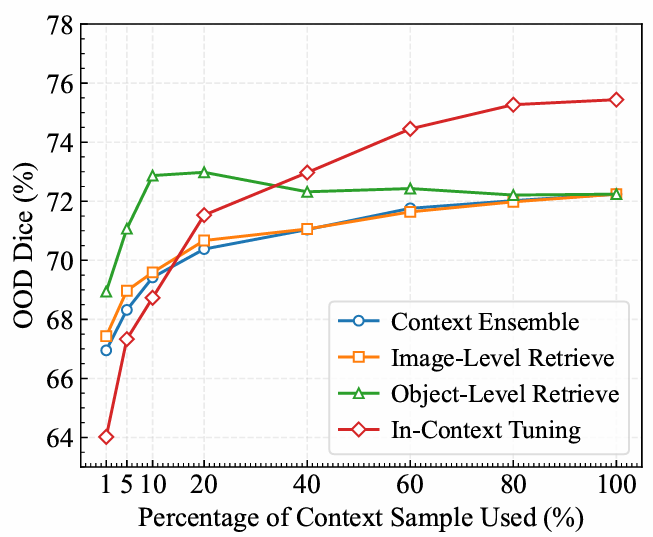
\includegraphics[width=0.8\linewidth]{fig/performance_comparison.png}
\caption{Comparative analysis of inference strategy performance across varying context sample utilization rates. The evaluation demonstrates four distinct approaches: Context Ensemble (blue circles), Image-Level Retrieve (orange squares), Object-Level Retrieve (green triangles), and In-Context Tuning (red diamonds). Results indicate that In-Context Tuning exhibits superior scalability, achieving progressive performance improvements from 64.2\% to 75.5\% Dice score as context sample usage increases from 1\% to 100\%. In contrast, the remaining three strategies demonstrate performance saturation around 72\% Dice score regardless of additional context availability, suggesting fundamental limitations in their ability to leverage increased reference information for enhanced segmentation quality.}
  \label{fig:performance_comparison}
\end{figure}
